\documentclass[a4paper,12pt]{report}

\usepackage{alltt, fancyvrb, url}
\usepackage{graphicx}
\usepackage[utf8]{inputenc}
\usepackage{float}
\usepackage{hyperref}

% Questo commentalo se vuoi scrivere in inglese.
\usepackage[italian]{babel}

\usepackage[italian]{cleveref}

\title{Relazione \\``Tank - Battle''}

\author{Tomas Ventrucci \\Riccardo Frascio \\Emanuele Martelli \\Lucrezia Rettori}
\date{10 Aprile 2023}


\begin{document}

\maketitle

\tableofcontents

\chapter{Analisi}

\section{Requisiti}
Il progetto si pone l’obiettivo di creare un videogioco dual player. I giocatori rappresentati da due carri armati si sfideranno cercando di abbattersi a vicenda. Il carro armato che rimane in vita vince. Per aumentare la varietà delle sfide, sarà possibile combattere con carri armati aventi diverse caratteristiche (velocità, potenza del colpo e vita) su mappe differenti.

\subsection*{Requisiti funzionali}
Il gioco dovrà occuparsi di gestire la partita degli utenti all’interno delle mappe di Tank-Battle. In particolare:
    \begin{itemize}
        \item il giocatore dovrà potersi muovere e sparare;
        \item la vita del nemico dovrà essere diminuita in conseguenza del colpo inflitto;
        \item la partita dovrà concludersi quando uno dei due carri armati avrà vita nulla;
        \item il giocatore dovrà essere in grado di capire lo stato della partita potendo visualizzare la propria vita e quella dell'avversario.
    \end{itemize}
\subsection*{Requisiti non funzionali}
\begin{itemize}
	\item Il gioco dovrà mantenere un profilo di prestazioni fluido e costante al variare dello stato e degli eventi di gioco.
\end{itemize}
\newpage
\section{Analisi e modello del dominio}
Una volta fatta partire l’applicazione, verrà presentato un menu nel quale si potrà scegliere tra:
\begin{itemize}
	\item iniziare una partita con la configurazione di default;
	\item entrare nella sezione tutorial;
	\item entrare nella sezione settings.
\end{itemize}
La configurazione di default darà modo di svolgere una partita in cui i giocatori avranno lo stesso tipo di carro armato.
Nella sezione tutorial sarà possibile visualizzare i comandi di gioco per entrambi i player e tornare al menu principale.
Nella sezione settings si potrà personalizzare la configurazione di gioco (scelta del tank per ogni giocatore e scelta della mappa).\\
Durante una partita i giocatori avranno la possibilità di muoversi all’interno della mappa e di sparare dei proiettili per cercare di abbattere l’avversario.
La mappa sarà composta da entità non attraversabili dai carri armati.
Ostacoli distruttibili saranno oggetto di studio per un’implementazione futura.
Quando il carro armato verrà colpito da un proiettile la sua vita dovrà diminuire e quando questa sarà nulla la partita dovrà terminare.
Conclusosi il gioco, Tank-Battle offrirà la possibilità di giocare un’altra partita con la stessa configurazione, di tornare al menu iniziale o di chiudere l’applicazione.
Prevediamo che l’implementazione di questo gioco presenterà, tra le altre, le seguenti difficoltà:
\begin{itemize}
	\item gestione delle collisioni tra le entità del gioco (muri, carri armati, proiettili);
	\item gestione della grafica in modo da rendere il gioco fluido e utilizzabile;
	\item gestione di mappe e carri armati differenti.
\end{itemize}
%
\chapter{Design}
\section{Architettura}
Tank-Battle è stato sviluppato utilizzando il pattern architetturale Model-View-Controller contaminato dal pattern Component in modo da sfruttare i vantaggi di entrambi.\\
Il pattern Component permette a una singola entità di estendersi su domini multipli senza accorparli in un’unica classe. Applicandolo al Model, abbiamo che ogni elemento del gioco risulta essere un gameObject. Ad ogni gameObject vengono aggiunti dei componenti, ognuno dei quali appartiene a un dominio specifico (moovement, collidable, ...). Ogni componente si aggiorna a seconda degli eventi generati dal mondo o dall’utente. L'utilità del pattern component sta nel poter costruire gameObject complessi utilizzando dei componenti semplici.\\
Dal punto di vista del pattern architetturale Model-View-Controller, i tre moduli sono descritti come segue: 
\begin{itemize}
	\item \textbf{Model}:
	il ruolo del ”Model” viene affidato all’insieme delle classi che sono contenute nel package model. In particolare da GameObject, World e GameState.
	\item \textbf{Controller}:
	il ruolo di “Controller” viene affidato all’insieme delle classi contenute nel package controller, in particolare all'interfaccia GameEngine che gestisce l’avanzamento del gioco aggiornando i componenti dei GameObject ed effettuando il render sulla View.
	\item \textbf{View}:
	Il ruolo di "View" viene affidato all’insieme delle classi contenute nel package view, in particolare all’interfaccia View, la quale descrive il concetto di controller di gestione dell'intefaccia grafica.
\end{itemize}
\newpage Con queste divisioni viene rispettata la modularità del pattern MVC potendone sfruttare i vantaggi. Se per esempio si desiderasse cambiare libreria grafica, si dovrebbero sostituire soltanto le implementazioni all’interno del package view.
	
\begin{figure}[H]
\centering{}
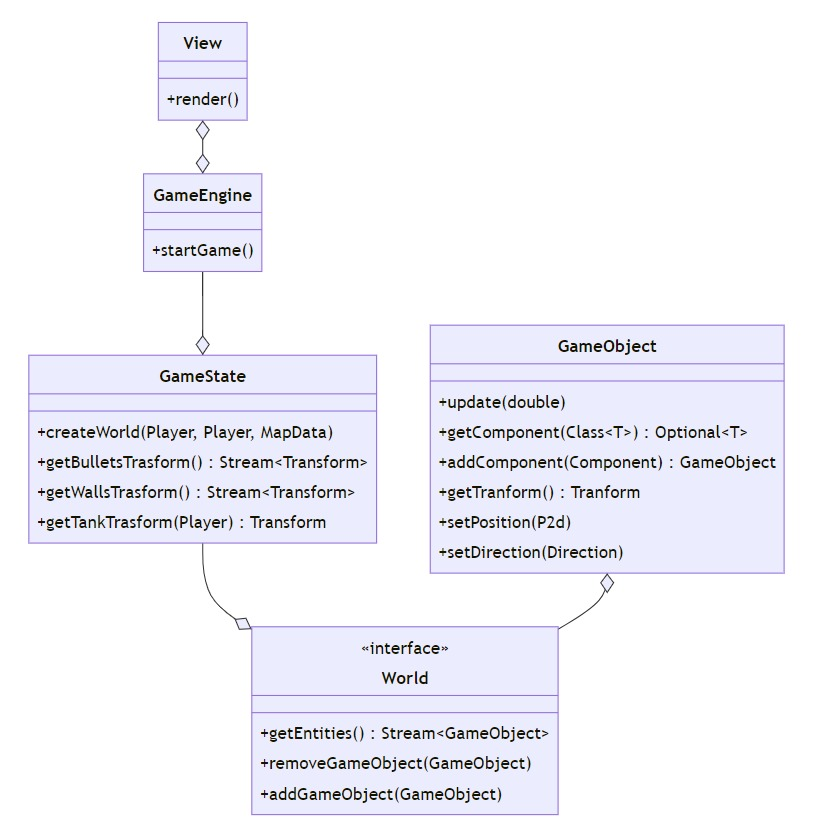
\includegraphics[width=1\textwidth]{img/MVC.jpg}
\caption{Schema UML architetturale di Tank-Battle.}
\label{img:analysis}
\end{figure}

\section{Design dettagliato}
%
\subsection*{Tomas Ventrucci}
%
\subsubsection*{Gestione dell’input}
%
\begin{figure}[H]
	\centering{}
	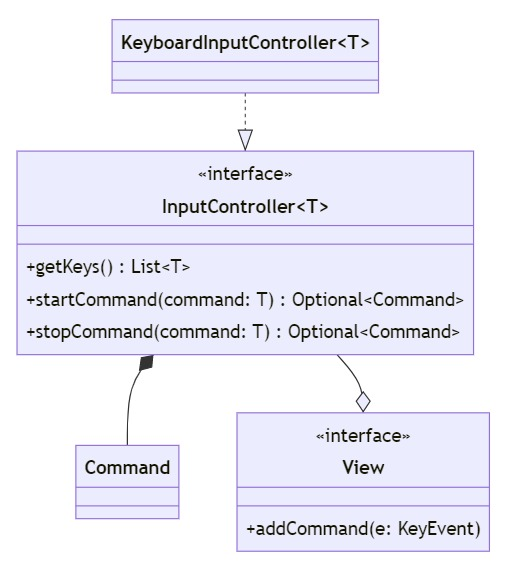
\includegraphics[scale=0.40]{img/input.jpg}
	\caption{Rappresentazione UML di InputController.}
	\end{figure}
%
\paragraph*{Problema} Prevedere la possibilità che l’input possa provenire non soltanto dalla tastiera del pc.
\paragraph*{Soluzione} Viene gestita un’interfaccia generica InputController che in base alla sorgente di input utilizzata avrà il compito di coordinare i comandi dati dall’utente, gestendo il concetto di inizio e fine di un comando. Nel nostro caso, viene implementata la classe KeyboardInputController. L’utilizzo di un’interfaccia generica ci consente inoltre di poter cambiare libreria grafica senza dover modificare il concetto generale espresso dall’interfaccia.
%
\newpage
\subsubsection*{Gestione dei comandi di gioco}
%
\begin{figure}[H]
	\centering{}
	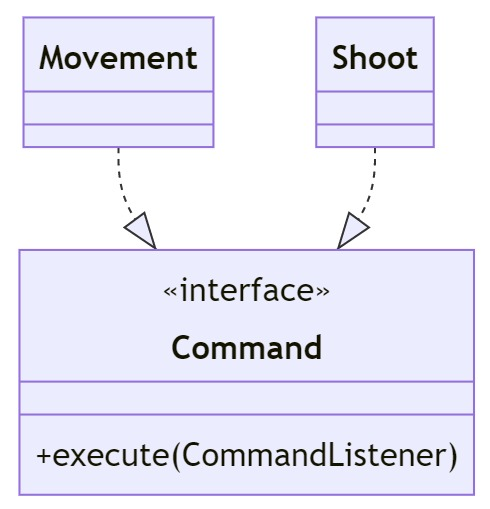
\includegraphics[scale=0.4]{img/command.jpg}
	\caption{Rappresentazione UML dell' interfaccia Command.}
	\label{img:strategy}
	\end{figure}
%	
\paragraph*{Problema} Scorporare l'intercettazione del comando dalla sua esecuzione.
%
\paragraph*{Soluzione} Utilizzo del Command pattern. Una volta che l’evento scaturito dalla pressione di un tasto viene intercettato dalla view, si notifica al contoller la presenza di un nuovo comando. Il controller si occuperà di chiamare l’esecuzione, senza però avere dettagli implementativi del comando. I comandi, infatti, sono incapsulati tramite l’apposita interfaccia Command. Nel nostro gioco si gestiscono due tipi di comandi tramite ereditarietà: moovement e shoot, entrambi utilizzati per far muovere il player e per consentirgli di sparare.
La struttura del Command pattern è composta da:
\begin{itemize}
	\item \textbf{Command}:
	l'interfaccia che definisce l’operazione da eseguire. In questo caso rappresentato da Command;
	\item \textbf{Concrete Command}:
	classe che implementa l’interfaccia Command e specifica la logica di esecuzione per una determinata richiesta. In questo caso rappresentato da Moovement e Shoot;
	\item \textbf{Receiver}:
	classe che contiene la logica vera e propria. I comandi gestiscono solo i dettagli di come una richiesta viene passata al receiver: infatti è il receiver che esegue il comando. Il reciever in questo caso è rappresentato dai diversi Component del GameObject;
	\item \textbf{Invoker}:
	classe che inizializza la richiesta. In questo caso rappresentato dalla view.
\end{itemize}
L’utilizzo del Command pattern facilita l’inserimento di nuovi comandi e la modifica di quelli esistenti.
%
\\ \\
\subsubsection*{Gestione del gameLoop}
%
\paragraph*{Problema} Gestire l'avanzamento del gioco.
%
\paragraph*{Soluzione} Tutta la logica del gioco è fondata su un ciclo perenne dal quale si esce soltanto se uno dei due carri armati viene distrutto. Ad ogni iterazione, vengono richiamate tutte le funzionalità del gioco nel seguente ordine:
\begin{itemize}
	\item \textbf{processInput}:
	si processano i vari comandi inseriti dagli utenti;
	\item \textbf{update}:
	vengono aggiornati i componenti del gioco;
	\item \textbf{render}:
	si ridisegna l’intera interfaccia di gioco aggiornata;
	\item \textbf{waitForNextFrame}:
	si mette in attesa il loop se l’esecuzione degli step precedenti è stata più rapida del periodo impostato.
\end{itemize}
Questo metodo ci dà la possibilità di descrivere in semplici passaggi tutto ciò che l’applicazione deve svolgere. Inoltre permette un’interazione fluida con l’utente.
Tale metodologia è quella che ci ha illustrato il Prof. A. Ricci ed è anche presente nel libro “Game programming patterns” di Robert Nystrom che abbiamo utilizzato come riferimento.
%
\newpage
\subsection*{Riccardo Frascio}
%
\subsubsection*{Creazione delle entità}
%
\begin{figure}[H]
	\centering{}
	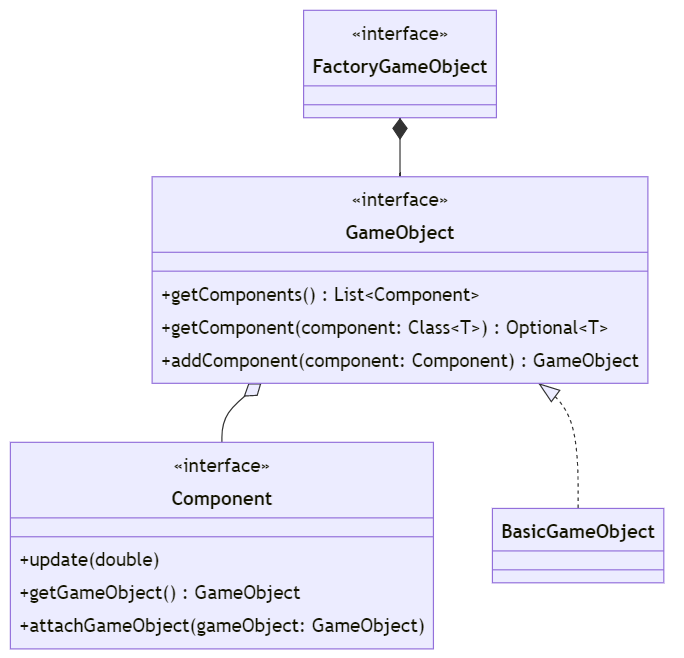
\includegraphics[scale=0.60]{img/gameObject.png}
	\caption{Rappresentazione UML della gestione dei GameObject.}
	\end{figure}
%
\paragraph*{Problema} Come poter gestire le diverse proprietà delle varie entità del gioco, come la vita, la velocità, le collisioni, o qualsiasi altra possibile caratteristica di un’entità di gioco.
\paragraph*{Soluzione} Per la creazione delle diverse entità è stato utilizzato il pattern \textbf{Component}, in modo tale che ogni GameObject abbia una lista di Component. Questo porta ad un’ottima estensibilità, potendo creare molto facilmente nuovi component e aggiungerli ai GameObject che lo necessitano.\\ 
I diversi GameObject verranno poi creati tramite una \textbf{Factory}, in cui ad ogni entità si aggiungono i vari component necessari.
%
\begin{figure}[H]
	\centering{}
	\includegraphics[scale=0.75]{img/component.png}
	\caption{Rappresentazione UML dell'architettura Component.}
	\label{img:strategy}
	\end{figure}
%
Per la distinzione tra le varie tipologie di entità sono stati poi creati diversi componenti rappresentanti le tipologie presenti, favorendo l’estensibilità potendo facilmente aggiungere un nuovo componente in caso di creazione di una ulteriore entità.
\newpage
\subsubsection*{Creazione di diverse tipologie di carri armati}
%
\begin{figure}[H]
	\centering{}
	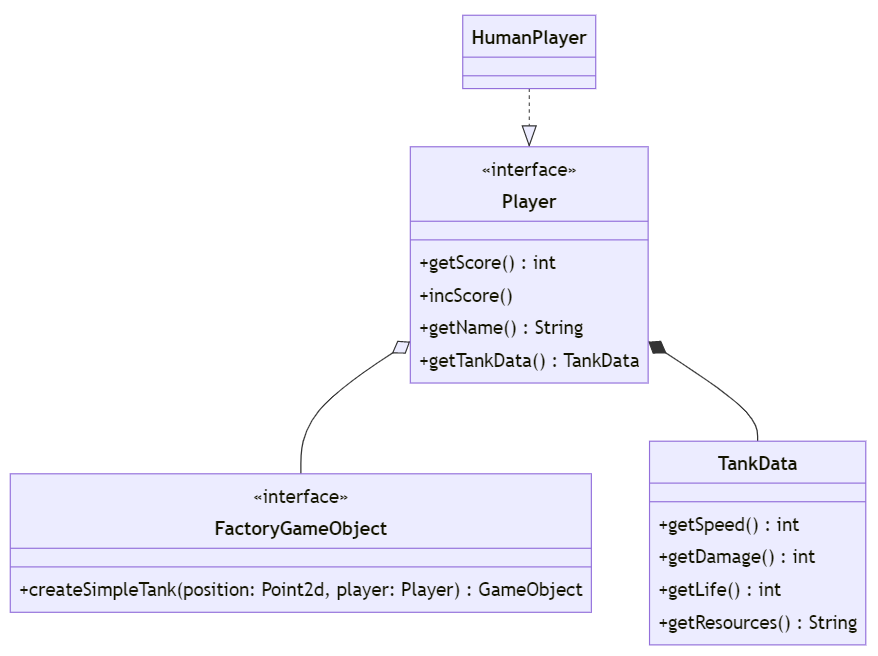
\includegraphics[scale=0.75]{img/tankData.png}
	\caption{Rappresentazione UML della gestione di carri armati differenti.}
	\label{img:strategy}
	\end{figure}
%	
\paragraph*{Problema} Come creare diverse tipologie di carri armati, con statistiche diverse, mantenendo facile la possibile aggiunta futura di nuove tipologie.
%
\paragraph*{Soluzione} Per la creazione di diverse tipologie di carri armati è stata fatta una classe TankData, la quale conterrà informazioni riguardanti le diverse caratteristiche di un carro armato, lette da un file xml, facilitando la futura aggiunta di eventuali nuovi tipi di cari armati. Un’istanza di TankData sarà poi contenuta dentro Player, il quale sarà associato ad un carro armato. Grazie a ciò, per la futura aggiunta di un nuovo tipo di carro armato sarà necessario solamente aggiungere una nuova istanza di tank dentro il file xml.
%
\newpage
\subsubsection*{Visualizzazione delle entità nella mappa}
%
\begin{figure}[H]
	\centering{}
	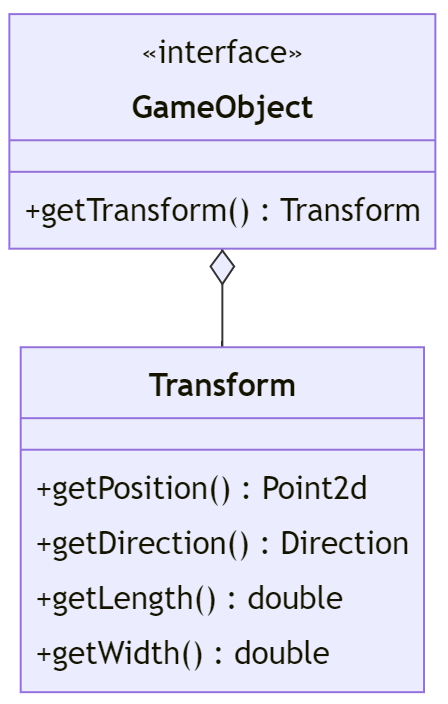
\includegraphics[scale=0.6]{img/transform.png}
	\caption{Rappresentazione UML dell'utilizza di Transform.}
	\label{img:strategy}
	\end{figure}
%
\paragraph*{Problema} Come poter rappresentare tutte le caratteristiche dei GameObject all’interno della mappa?
%
\paragraph*{Soluzione} Per fare ciò è stata realizzata una classe Transform, la quale sarà contenuta in ogni GameObject. Questa classe è stata creata per raggruppare tutte le informazioni necessarie per rappresentare un’entità all’interno di una mappa, quindi con i campi di posizione, direzione, lunghezza e altezza. Questo permette di ottenere molto più velocemente tutte le informazioni necessarie per gestire collisioni, movimenti, e rappresentazione grafica.\\
Questo limita anche la visibilità della View, in quanto non riceve informazioni riguardanti i GameObject, ma riceve dal controller solamente i Transform associati a questi ultimi.
\newpage
\subsubsection*{Gestione inizio e fine partita}
%
\begin{figure}[H]
	\centering{}
	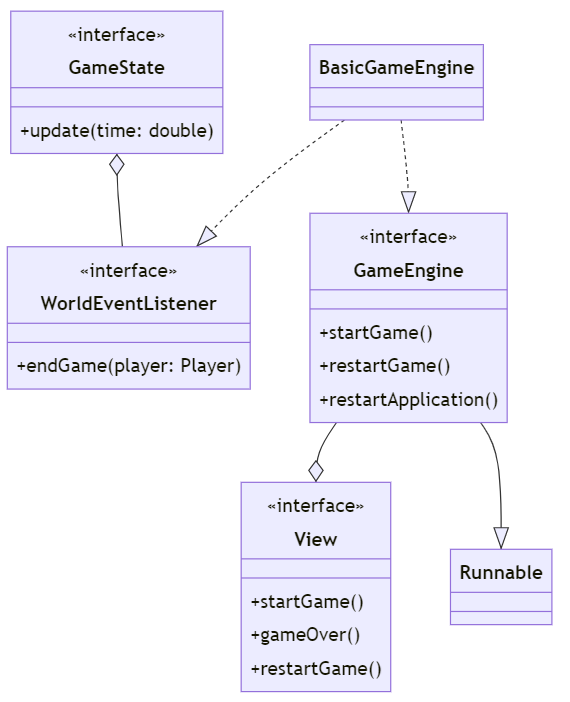
\includegraphics[scale=0.8]{img/runnable.png}
	\caption{Rappresentazione UML per logica di StartGame e GameOver.}
	\label{img:strategy}
	\end{figure}
%
\paragraph{} Per la gestione della partita è stato utilizzato un thread separato, il quale viene chiamato appena si inizia una nuova partita e terminerà con la morte di un carro armato, e dunque con la fine del loop. La fine di una partita verrà notificata al controller grazie al WorldEventListerner, il quale viene implementato dal BasicGameEngine, utilizzando il pattern \textbf{observer}, in maniera tale da limitare la visione del controller da parte del model solamente al WorldEventListerner.\\
Finita una partita, l’utente potrà scegliere se rigiocarne un’altra, richiamando così i metodi restartGame() di View e GameEngine , il quale creerà un nuovo thread, facendo ripartire il loop, oppure potrà tornare al menu, azzerando così lo score e istanziando un nuovo thread ma che partirà solamente iniziando un’altra partita.
%
\newpage
\subsection*{Emanuele Martelli}
%
\subsubsection*{Organizzazione del model}
%
\begin{figure}[H]
	\centering{}
	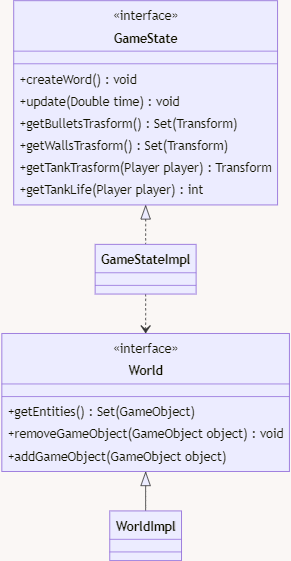
\includegraphics[scale=0.9]{img/gameState.png}
	\caption{Rappresentazione UML dell' architettura del Model.}
	\end{figure}
%
\paragraph{} Il model è stato in due principali classi identificate entrambi da delle interfacce, dove la prima ha il compito di gestire tutte le operazioni che gli vengono notificate dal controller e la seconda ha il compito di immagazzinare tutti i dati. Questa divisione non viola il single responsibility e dà la possibilità di estendere entrambi le classi con semplicità.
%
\begin{figure}[H]
	\centering{}
	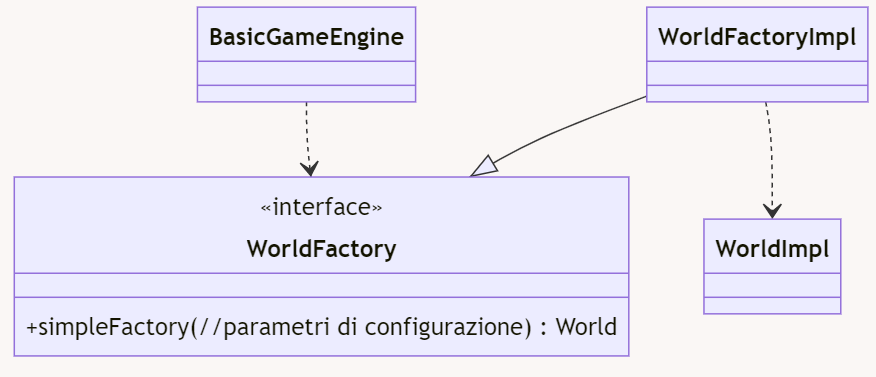
\includegraphics[scale=0.60]{img/worldFactory.png}
	\caption{Rappresentazione UML della creazione del world.}
	\end{figure}
%
\paragraph{} Successivamente ho deciso di dare la responsabilità di creare dei nuovi World a una classe a parte, sempre per rendere più facile una possibile espansione.
%
\begin{figure}[H]
	\centering{}
	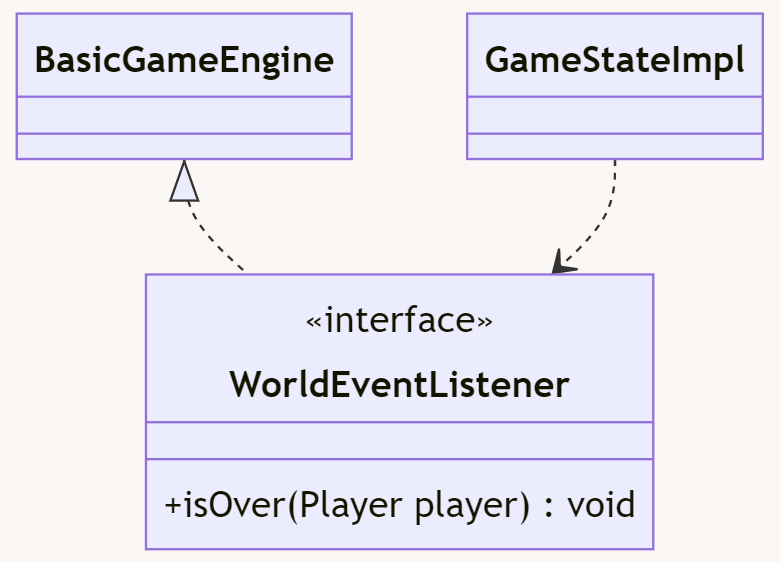
\includegraphics[scale=0.60]{img/worldEventListener.png}
	\caption{Rappresentazione UML listener per il world.}
	\end{figure}
%
\paragraph*{Problema} Trovare un modo per far comunicare il model con il controller evitando cicli di dipendenze e senza violare l’MVC.
\paragraph*{Soluzione} Creazione di un obsever che si mette in mezzo tra il model e il controller, così si può ampliare facilmente e si limita anche la visibilità non dando al model la visione dell’intero controller.
%
\begin{figure}[H]
	\centering{}
	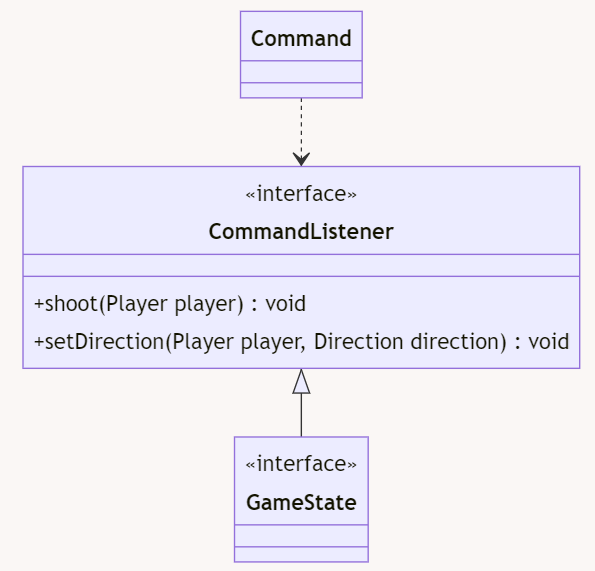
\includegraphics[scale=0.75]{img/commandListener.png}
	\caption{Rappresentazione UML listener per il model.}
	\label{img:strategy}
	\end{figure}
%
\paragraph{} Ho utilizzato una soluzione simile anche per i command, così da evitare di passare tutto il model ai command ma solo una censura con solo i metodi che i command hanno bisogno.
\newpage
\subsubsection*{Lettura da file}
%
\begin{figure}[H]
	\centering{}
	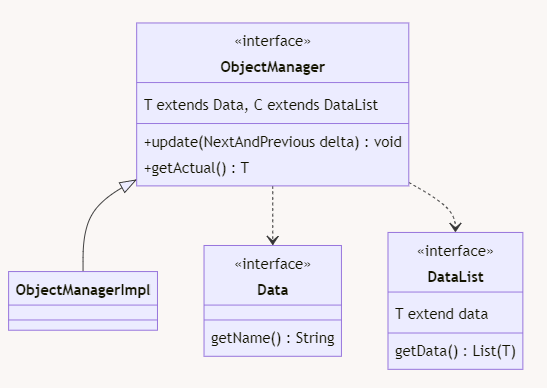
\includegraphics[scale=0.85]{img/objectManager.png}
	\caption{Rappresentazione UML dell'architettura per leggere file.}
	\label{img:strategy}
	\end{figure}
%	
\paragraph*{Problema} Come creare dei manager per leggere informazioni sulle mappe e sui carrarmati da file.
%
\paragraph*{Soluzione} Creare una classe ObjectManager che generalizza entrambi così che a seconda di come viene creato capisce già che tipo di dati andrà a leggere. E creazione di Data e Datalist<T extend Data> due interfacce che generalizzano i principali tipi di informazioni presenti nei file. Così facendo se un giorno si ha bisogno di un altro tipo di manager per tipi diversi di file, basta creare un’altra implementazione di ObjetctManager, mentre se si ha bisogno di leggere tipi di data diversi ma da uno stesso tipo di file, basta creare altre implementazioni di Data e DataList.
%
\newpage
\subsection*{Lucrezia Rettori}
%
\subsubsection*{Components}
%
\begin{figure}[H]
    \centering{}
    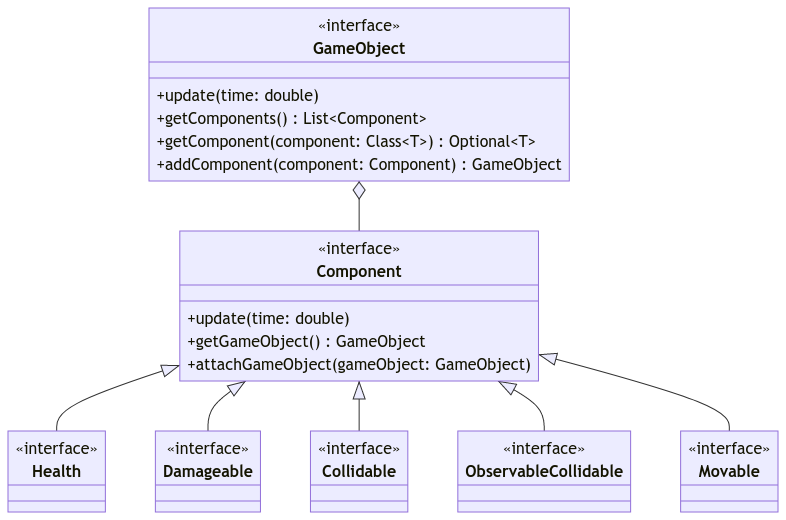
\includegraphics[width=\textwidth]{img/Components.png}
    \caption{Schema UML dell'architettura generale dei Component.}
\end{figure}
%
\paragraph*{Problema}
Gestire il comportamento dei diversi oggetti presenti nel gioco in modo componibile, evitando di creare classi con troppe responsabilità.
\paragraph*{Soluzione}
Già dopo la prima analisi del progetto si è potuto notare che i diversi oggetti in gioco mostravano alcuni comportamenti in comune, come ad esempio muoversi, collidere o ricevere danno in relazione a eventi esterni.
Questi comportamenti sono stati quindi divisi in componenti che singolarmente vengono gestiti da \texttt{GameObject}.
Questo consente sia di poterli applicare a qualsiasi tipo di oggetto, quindi di riusare codice comune, sia di poter agire sul singolo comportamento senza dover intaccare ogni volta gli oggetti stessi (se ad esempio si dovesse avere la necessità di modificare il comportamento di un particolare oggetto in caso di collisione, si potrebbe facilmente creare un nuovo componente con un comportamento diverso da agganciargli, anziché dover agire su ogni oggetto coinvolto).
Il comportamento complesso dei vari oggetti in gioco è quindi definito dalla composizione di differenti comportamenti atomici suddivisi in componenti.
Questo approccio è stato scelto a discapito dell'ereditarietà, che eventualmente si sarebbe potuta applicare avendo sempre l'interfaccia \texttt{GameObject} ma implementando varie sottoclassi associate agli oggetti in gioco. Ciò avrebbe portato alla necessità di creare una nuova sottoclasse per ogni differenza di comportamento fra gli oggetti, rischiando un elevato numero di sottoclassi e obbligando varie ripetizioni di codice evitabili ricercando invece la composizione dei singoli comportamenti.

Nello specifico, la composizione dei comportamenti avviene agganciando i componenti attraverso il metodo \texttt{addComponent()} proprio del \texttt{GameObject}. In aggiunta, ciascun componente implementa il suo comportamento tramite l'implementazione dei metodi \texttt{update()} e \texttt{attachGameObject()}, che vengono rispettivamente chiamati da \texttt{GameObject} a fronte del proprio metodo \texttt{update()} e di \texttt{addComponent()}.
%
\begin{figure}
    \centering{}
    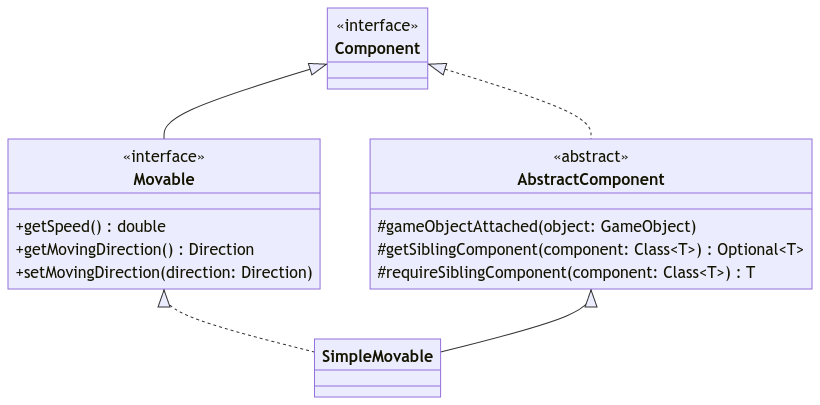
\includegraphics[width=\textwidth]{img/SimpleMovable.png}
    \caption{Schema UML dell'architettura del Component SimpleMovable.}
    \label{fig:simple-movable}
\end{figure}
%

La classe astratta \texttt{AbstractComponent} gestisce azioni comuni a tutte le sottoclassi, implementando l'interfaccia \texttt{Component} stessa. In particolare, si fa uso del pattern \textbf{Template Method} per l'implementazione del metodo \texttt{attachGameObject}, per consentire alle sottoclassi di eseguire del comportamento quando un componente viene agganciato al \texttt{GameObject} tramite il metodo \texttt{gameObjectAttached()}.

In \Cref{fig:simple-movable} è possibile ad esempio vedere la gestione della mobilità degli oggetti: non tutti hanno la possibilità di spostarsi, quelli che possono hanno il relativo componente \texttt{SimpleMovable}, che gestisce il comportamento attraverso i metodi dichiarati dall'interfaccia \texttt{Movable}.
%
\newpage
%
\subsubsection*{Gestione delle collisioni}
%
\begin{figure}[H]
    \centering{}
    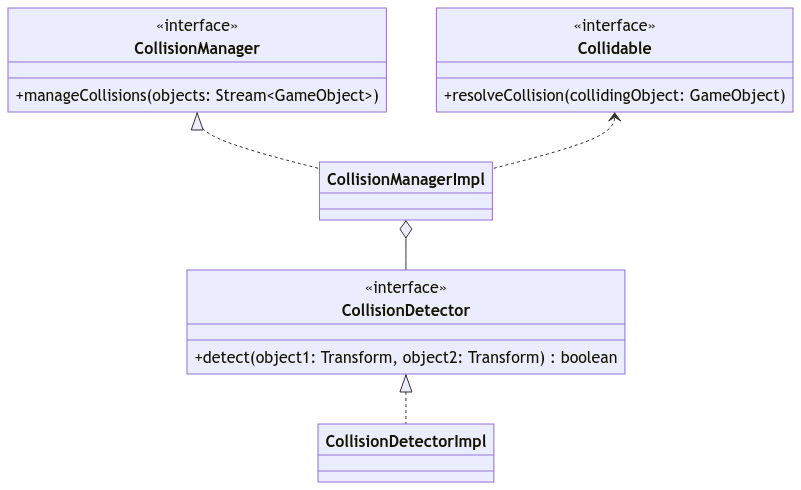
\includegraphics[width=\textwidth]{img/Collisions.png}
    \caption{Schema UML della gestione delle collisioni.}
\end{figure}
%
\paragraph*{Problema}
Rilevare le collisioni indipendentemente dall'entità degli oggetti in contatto e dalla loro situazione attuale al momento dell'impatto.
\paragraph*{Soluzione}
Si è deciso di separare la rilevazione delle collisioni e la gestione delle stesse in due interfacce diverse, per garantire una divisione netta delle responsabilità.

La difficoltà primaria consisteva nel riuscire a riconoscere due oggetti in collisione in qualunque momento durante il gioco e ad agire in merito secondo regole ben definite.

La classe che implementa i metodi relativi alla gestione della collisione, quindi quelli dell'interfaccia \texttt{CollisionManager}, si occupa di filtrare gli oggetti in gioco finendo per considerare unicamente gli oggetti che posseggono il componente \texttt{Collidable}, proprio degli oggetti riconosciuti come tangibili.
Su questi ultimi entra in gioco la classe relativa alla rilevazione della collisione, quindi quella che implementa i metodi dell'interfaccia \texttt{CollisionDetector}, che, ricevute le \texttt{Transform} associate ai \texttt{Collidable}, si occupa di verificare se queste sono in collisione e, in caso, ne lascia la gestione al \texttt{CollisionManagerImpl}, il quale richiama il metodo \texttt{resolveCollision()} sui singoli oggetti.
In base al tipo di oggetto si ricercano reazioni diverse alla collisione, e ciò si è potuto ottenere sfruttando nuovamente la gestione dei diversi comportamenti attraverso i componenti: in base alle necessità è stato possibile agganciare ai vari oggetti in gioco comportamenti diversi in caso di contatto: dover ricevere danno (attraverso i componenti \texttt{Damageable} e \texttt{DealDamageOnCollision}), dover sparire (attraverso il componente \texttt{DestroyOnCollision} che agisce sul componente \texttt{Health}) o dover ricevere un contraccolpo (attraverso il componente \texttt{KnockBack}, che sfrutta le conoscenze su posizione, direzione e velocità dell'oggetto per calcolare in che direzione spostarlo successivamente alla collisione).
Dato che ci sono più componenti che gestiscono il comportamento a seguito di una collisione, si è deciso di creare una classe astratta (\texttt{CollisionHandlingComponent}, visibile anticipando lo schema in \Cref{fig:health} e in \Cref{fig:knock-back}) che gestisce la sottoscrizione all'evento dei suddetti.
%
\begin{figure}[H]
    \centering{}
    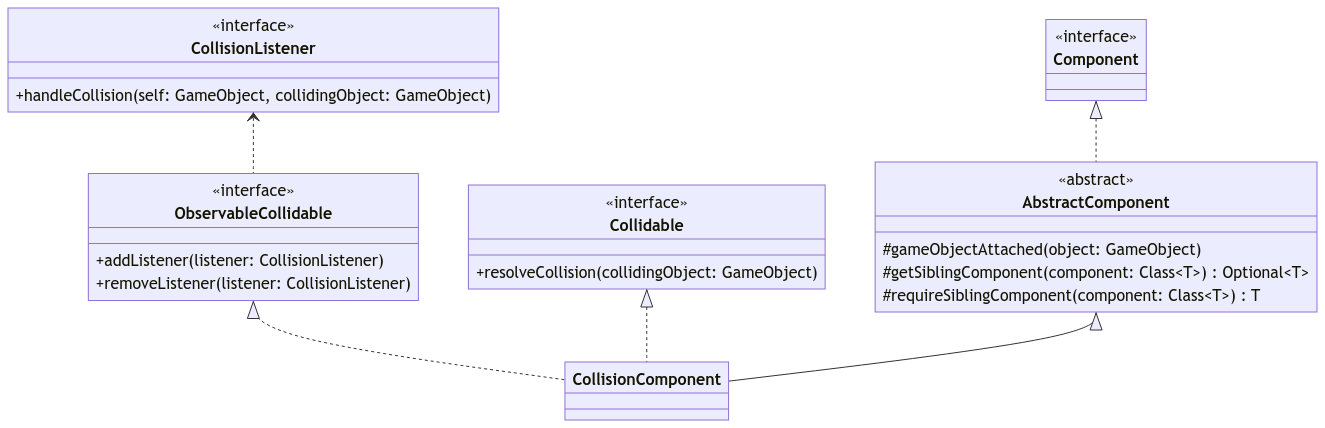
\includegraphics[width=\textwidth]{img/CollisionComponent.png}
    \caption{Schema UML della rappresentazione dell'applicazione del pattern Observer.}
\end{figure}
%
\paragraph*{Problema}
Gestire gli effetti relativi alle collisioni fra tutti gli oggetti presenti in gioco, evitando forti dipendenze o ripetizioni di codice.
\paragraph*{Soluzione}
Si è deciso di utilizzare il pattern \textbf{Observer} per gestire le collisioni, così da lasciare la responsabilità della gestione dell'evento ai singoli oggetti interessati.
%
L'applicazione di questo particolare pattern poggia sulle due interfacce \texttt{ObservableCollidable} e \texttt{Collidable}, che insieme rappresentano la parte \textit{observable} del pattern: la prima si occupa di registrare e rimuovere i singoli listener a cui l'interfaccia \texttt{Collidable} fa riferimento per la notifica agli \textit{observer} (rappresentati dai \texttt{CollisionListener}).
Si è optato per questa divisione dei ruoli fra \texttt{ObservableCollidable} e \texttt{Collidable} per seguire il principio di \textit{interface segregation} ed evitare così una dipendenza che sarebbe difficile da trattare a seguito di una possibile evoluzione futura del codice. 
I \texttt{CollisionListener}, una volta notificati dell'evento attraverso il metodo \texttt{handleCollision()}, lo gestiscono in modo appropriato a seconda dell'implementazione concreta diversificata fra i vari componenti.
In \Cref{fig:health} e in \Cref{fig:knock-back} è possibile visualizzarne degli esempi.
%
\begin{figure}[H]
    \centering{}
    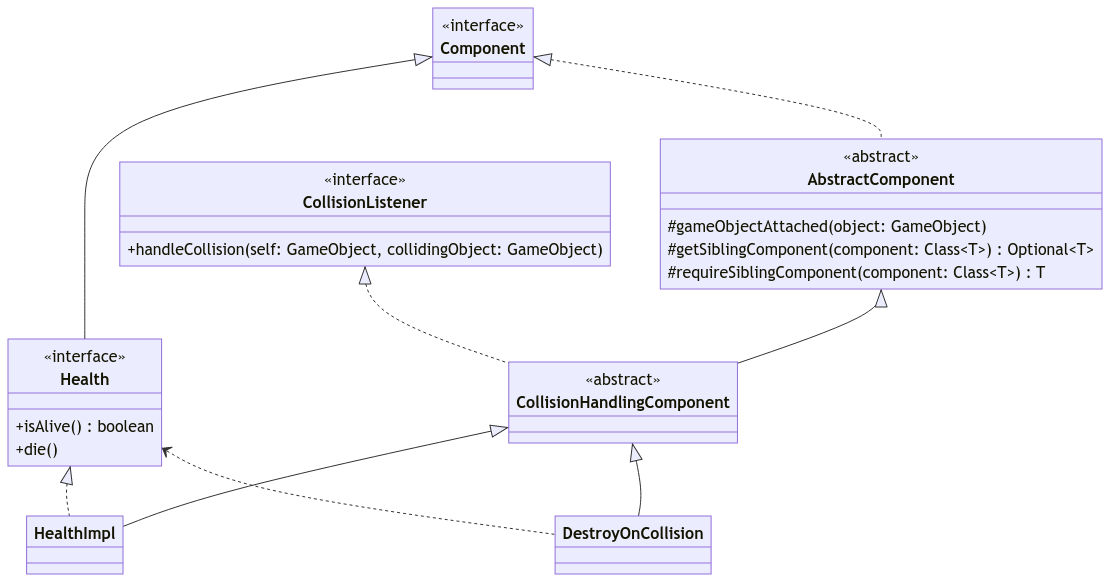
\includegraphics[width=\textwidth]{img/Health.png}
    \caption{Schema UML della gestione della vita degli oggetti.}
    \label{fig:health}
\end{figure}
%
\begin{figure}[H]
    \centering{}
    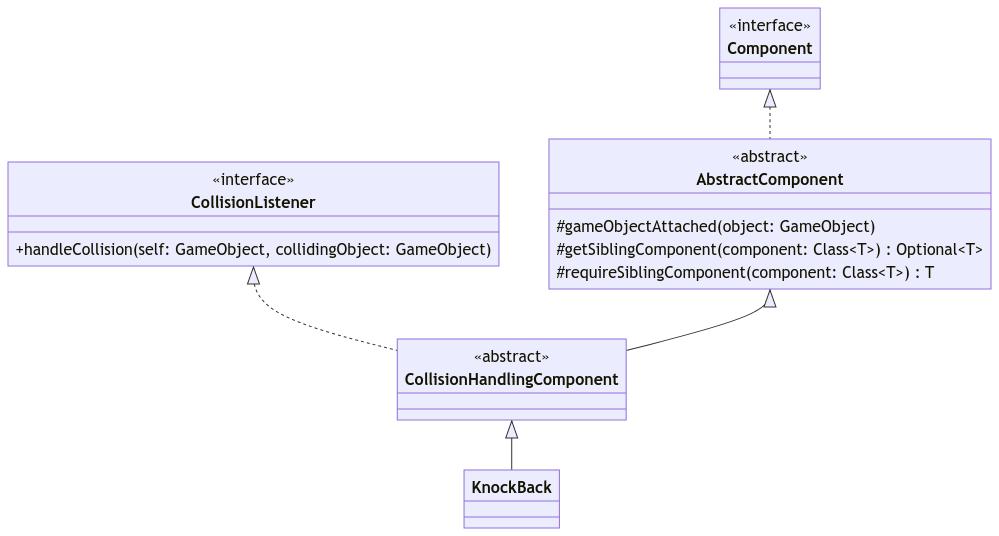
\includegraphics[width=\textwidth]{img/KnockBack.png}
    \caption{Schema UML della gestione del contraccolpo in caso di collisione.}
    \label{fig:knock-back}
\end{figure}
%
Il \textit{concrete observable} in questa trasposizione del pattern è rappresentato dal \texttt{CollisionComponent}, che informa i \textit{concrete observers} sfruttando l'operazione di notifica ereditata dall'\textit{observable}.
Per \textit{concrete observers} si intendono tutti gli oggetti che implementano il \texttt{CollisionListener}, come le classi \texttt{KnockBack}, \texttt{DestroyOnCollision} e \texttt{DealDamageOnCollision}, le quali mostrano tre modi differenti di comportarsi in relazione alla collisione avvenuta e sono ugualmente agganciabili a qualunque oggetto per determinarne il comportamento proprio.
%
\chapter{Sviluppo}
\section{Testing automatizzato}

Per effettuare i test abbiamo utilizzato JUnit 5.
\\I test che abbiamo effettuato sono:
\begin{itemize}
	\item \textbf{CommandTest}, questa classe verifica la creazione dei comandi simulando l'input dell'utente.
	\item \textbf{ObjectManagerTest}, questa classe testa la lettura del file xml e che l'ObjectManager restituisca il giusto valore simulando la richiesta dell'utente.
	\item \textbf{GameObjectTest}, questa classe verifica le principali funzionalità dei GameObject.
    \item \textbf{ModelTest}, questa classe esamina le funzionalità basilari del model.
    \item \textbf{CollisionDetectorImplTest}, testata la corretta presenza o assenza di collisioni passando varie \texttt{Transform} per simulare le casistiche.
    \item \textbf{CollisionComponentTest}, testato il corretto funzionamento in relazione all'inserimento e rimozione dei listener relativi alle collisioni.
\end{itemize}
Non sono stati eseguiti test sulle funzionalità grafiche perchè il render dei GameObject dipende dal corretto funzionamento dei singoli componenti che abbiamo testato come sopra descritto. Il miglior test che si può sfruttare è l'esecuzione dell'applicazione.
\newpage
\section{Metodologia di lavoro}
La prima fase del nostro lavoro è stata quella di progettazione discutendo l'architettura generale del gioco. Fra le varie possibilità. la scelta è ricaduta sul pattern MVC visto in classe.
Abbiamo creato lo scheletro dell'applicazione e in seguito, in base alle suddivisioni, ognuno di noi ha pensato più nel dettaglio a come poter gestire la propria parte. Di conseguenza abbiamo svolto un briefing per esporre le idee e raccoglierne di nuove.\\
Durante lo sviluppo del codice siamo riusciti a lavorare in parallelo, utilizzando il DVCS come visto in classe. Ognuno di noi ha fatto un clone del repository, creato il proprio branch e lo ha tenuto aggiornato tramite pull e push.\\
Al termine dell’implementazione di ogni parte del gioco, ci siamo ritrovati per decidere come accorparla alla struttura principale. Infine abbiamo riguardato tutto il codice per sistemare gli ultimi dettagli.
%
\\ \\ 
\subsection*{Tomas Ventrucci}
In autonomia mi sono occupato di:
\begin{itemize}
	\item Gestione dell’input \\(package it.unibo.tankbattle.common.input)
	\item Implementazione dei comandi \\(package it.unibo.tankbattle.common.input)
	\item Gestione dell’interfaccia grafica \\(package it.unibo.tankbattle.view)
	\item Implementazione del GameLoop \\(package it.unibo.tankbattle.controller)
	\item Gestione del launcher \\(package it.unibo.tankbattle classi TankBattle e Main)
	\item Gestione dell’audio \\(package it.unibo.tankbattle.view.impl.javafx.controller GameController) \\ \\ \\
\end{itemize} 
In collaborazione mi sono occupato:
\begin{itemize}
	\item Con Riccardo Frascio:
		\begin{itemize}
			\item Gestione del GameController.
			\item Gestione del GameEngine.
		\end{itemize}
	\item Con Emanuele Martelli:
		\begin{itemize}
			\item Lettura da file xml.
			\item Gestione del GameSetup.
            \item Gestione del GameEngine.
		\end{itemize}
\end{itemize}
\subsection*{Riccardo Frascio}
In autonomia mi sono occupato di:
\begin{itemize}
	\item Creazione GameObject, GameObjectFactory e la loro implementazione (package it.unibo.tankbattle.model.gameobject)
	\item Creazione del pattern component, classi Component e abstractComponent (package it.unibo.tankbattle.model.gameobject.api.component)
    \item Implementazione delle classi Wall, Tank, Bullet \\
(package it.unibo.tankbattle.model.gameobject.api.component)
	\item Gestione del thread per l’inizio, fine e restart della partita (package it.unibo.tankbattle.controller)
    \item Creazione dello sprite per lo sparo e l’esplosione del proiettile (package it.unibo.tankbattle.view.impl.javafx.controller)
    \item Gestione di un resize diagonale e proporzionato nella schermata di gioco (package it.unibo.tankbattle.view.impl.javafx.controller)
\end{itemize}
In collaborazione mi sono occupato:
\begin{itemize}
	\item Con Emanuele Martelli:
        \begin{itemize}
	\item Gestione del rapporto tra GameObject-World-GameState, di come trasmettere le informazioni e mantenerle il più incapsulate possibile.
    \item Gestione del GameEngine.
        \end{itemize}
        \item Con Tomas Ventrucci:
        \begin{itemize}
	\item Gestione del GameController.
    \item Gestione del GameEngine.
        \end{itemize}
\end{itemize}
\subsection*{Emanuele Martelli}
In autonomia mi sono occupato di:
\begin{itemize}
	\item Creazione di World e WorldFactory e le loro implementazioni \\(package it.unibo.tankbattle.model.world)
	\item Creazione e implementazione del GameState\\ (package it.unibo.tankbattle.model.gamestate)
    \item Utilizzo del pattern Observer WorldEventListener\\
(package it.unibo.tankbattle.model.gamestate.api)
    \item Creazione delle interfacce Data e DataList \\
(package it.unibo.tankbattle.model.gamesetup.api)
    \item Creazione di Line e Position per la lettura da file \\
(package it.unibo.tankbattle.model.gamesetup.impl)
    \item Creazione dell’interfaccia ObjectManager \\
(package it.unibo.tankbattle.controller.api)
    \item Creazione di CommandEventListener \\
(package it.unibo.tankbattle.model.gamestate.api)
\end{itemize}
In collaborazione mi sono occupato:
\begin{itemize}
	\item Riccardo Frascio
    \begin{itemize}
        \item Gestione del rapporto tra GameObject-World-GameState, di come trasmettere le informazioni e mantenerle il più incapsulate possibile
        \item Gestione del GameEngine
    \end{itemize}
    \item Tomas Ventrucci
    \begin{itemize}
        \item La lettura da file (read di ObjectManagerImpl)
        \item Gestione di GameEngine 
    \end{itemize}
\end{itemize}
\subsection*{Lucrezia Rettori}
In autonomia mi sono occupata di:
\begin{itemize}
    \item Creazione dei componenti per la suddivisione dei comportamenti degli oggetti, in modo che fossero poi componibili su GameObject \\(package it.unibo.tankbattle.model.gameobject.api.component e\\ it.unibo.tankbattle.model.gameobject.impl.component).
    \item Gestione della parte relativa alle collisioni di tutti gli oggetti in gioco \\(package it.unibo.tankbattle.model.collision).
    \item Inserimento dei dati relativi alla creazione delle mappe all'interno del file \texttt{mapConfig.xml} (package it.unibo.tankbattle.resources.config).
\end{itemize}
%
\newpage
\section{Note di sviluppo}
\subsection*{Tomas Ventrucci}
\subsubsection*{Interfaccia con Generics e Optional}
\begin{itemize}
    \item Permalink: \url{https://github.com/Yaboku19/tank-battle-OOP/blob/1f2c1cade86d41b817c4a81ccefcc3ffbda18d65/src/main/java/it/unibo/tankbattle/common/input/api/InputController.java#L3-L29}
\end{itemize}
\subsubsection*{Interfaccia funzionale}
\begin{itemize}
    \item Permalink: \url{https://github.com/Yaboku19/tank-battle-OOP/blob/1f2c1cade86d41b817c4a81ccefcc3ffbda18d65/src/main/java/it/unibo/tankbattle/common/input/api/Command.java#L3-L135}
\end{itemize}
\subsubsection*{Utilizzo di Lambda expression}
\begin{itemize}
    \item Permalink: \url{https://github.com/Yaboku19/tank-battle-OOP/blob/1f2c1cade86d41b817c4a81ccefcc3ffbda18d65/src/main/java/it/unibo/tankbattle/view/impl/javafx/controller/ViewController.java#L60-L68}
\end{itemize}
\subsubsection*{Utilizzo della libreria JavaFX}
\begin{itemize}
    \item Permalink: \url{https://github.com/Yaboku19/tank-battle-OOP/blob/1f2c1cade86d41b817c4a81ccefcc3ffbda18d65/src/main/java/it/unibo/tankbattle/view/impl/javafx/controller/SettingsController.java#L3-L231}
\end{itemize}
\newpage
\subsection*{Riccardo Frascio}
\subsubsection*{Utilizzo di stream, optional e metodo generico}
\begin{itemize}
    \item Permalink: \url{https://github.com/Yaboku19/tank-battle-OOP/blob/a32378ed51c4aed2abbe4c38db905b447b6f0246/src/main/java/it/unibo/tankbattle/model/gameobject/impl/object/BasicGameObject.java#L56-L61}
\end{itemize}
\subsubsection*{Utilizzo di lambda e libreria JavaFx}
\begin{itemize}
    \item Permalink: \url{https://github.com/Yaboku19/tank-battle-OOP/blob/a32378ed51c4aed2abbe4c38db905b447b6f0246/src/main/java/it/unibo/tankbattle/view/impl/javafx/controller/ViewController.java#L305-L314}
\end{itemize}
\subsubsection*{Utilizzo di lambda}
\begin{itemize}
    \item Permalink: \url{https://github.com/Yaboku19/tank-battle-OOP/blob/a32378ed51c4aed2abbe4c38db905b447b6f0246/src/main/java/it/unibo/tankbattle/view/impl/javafx/controller/GameController.java#L158-L159}
    \item Permalink: \url{https://github.com/Yaboku19/tank-battle-OOP/blob/a32378ed51c4aed2abbe4c38db905b447b6f0246/src/main/java/it/unibo/tankbattle/view/impl/javafx/controller/GameController.java#L309-L312}
    \item Permalink: \url{https://github.com/Yaboku19/tank-battle-OOP/blob/a32378ed51c4aed2abbe4c38db905b447b6f0246/src/main/java/it/unibo/tankbattle/model/gameobject/impl/object/BasicGameObject.java#L40-L42}
\end{itemize}
\newpage
\subsection*{Emanuele Martelli}
\subsubsection*{Utilizzo di generici}
\begin{itemize}
    \item Permalink: \url{https://github.com/Yaboku19/tank-battle-OOP/blob/a32378ed51c4aed2abbe4c38db905b447b6f0246/src/main/java/it/unibo/tankbattle/controller/impl/ObjectsManagerImpl.java#L35-L57}
\end{itemize}
\subsubsection*{Uso di lambda expression e Stream} 
\begin{itemize}
    \item Permalink: \url{https://github.com/Yaboku19/tank-battle-OOP/blob/a32378ed51c4aed2abbe4c38db905b447b6f0246/src/main/java/it/unibo/tankbattle/model/gamestate/impl/GameStateImpl.java#L59-L63}
    \item Permalink: \url{https://github.com/Yaboku19/tank-battle-OOP/blob/a32378ed51c4aed2abbe4c38db905b447b6f0246/src/main/java/it/unibo/tankbattle/model/gamesetup/impl/MapData.java#L80-L86}
\end{itemize}
\subsubsection*{Uso di nuove annotazioni}
\begin{itemize}
    \item Permalink: \url{https://github.com/Yaboku19/tank-battle-OOP/blob/a32378ed51c4aed2abbe4c38db905b447b6f0246/src/main/java/it/unibo/tankbattle/model/gamesetup/impl/MapData.java#L17-L32}
\end{itemize}
\subsubsection*{Interfaccia funzionale}
\begin{itemize}
    \item Permalink: \url{https://github.com/Yaboku19/tank-battle-OOP/blob/a32378ed51c4aed2abbe4c38db905b447b6f0246/src/main/java/it/unibo/tankbattle/controller/api/ObjectsManager.java#L10-L22}
\end{itemize}
%
\newpage
\subsection*{Lucrezia Rettori}
\subsubsection*{Utilizzo di \texttt{Stream} e lambda expressions}
\begin{itemize}
    \item Permalink: \url{https://github.com/Yaboku19/tank-battle-OOP/blob/15dd1d5c7221fae9293eac736127a15fa72e7c31/src/main/java/it/unibo/tankbattle/model/collision/impl/CollisionManagerImpl.java#L28-L60}
    \item Permalink: \url{https://github.com/Yaboku19/tank-battle-OOP/blob/15dd1d5c7221fae9293eac736127a15fa72e7c31/src/main/java/it/unibo/tankbattle/model/collision/impl/CollisionDetectorImpl.java#L21-L40}
\end{itemize}
\subsubsection*{Utilizzo di interfacce funzionali}
\begin{itemize}
	\item Permalink: \url{https://github.com/Yaboku19/tank-battle-OOP/blob/15dd1d5c7221fae9293eac736127a15fa72e7c31/src/main/java/it/unibo/tankbattle/model/gameobject/impl/component/KnockBack.java#L57-L78}
\end{itemize}
\subsubsection*{Utilizzo di \texttt{Optional} e generici bounded}
\begin{itemize}
	\item Permalink: \url{https://github.com/Yaboku19/tank-battle-OOP/blob/15dd1d5c7221fae9293eac736127a15fa72e7c31/src/main/java/it/unibo/tankbattle/model/gameobject/impl/component/AbstractComponent.java#L48-L72}
\end{itemize}
%
\chapter{Commenti finali}
\section{Autovalutazione e lavori futuri}
\subsection*{Tomas Ventrucci}
Sono contento e soddisfatto del risultato ottenuto. L’idea di sviluppare un videogioco mi incuriosiva e mi intimoriva allo stesso tempo perché non avevo mai svolto un progetto così strutturato. Questo mi ha dato la spinta per mettermi totalmente in gioco cercando di trovare soluzioni per ogni problema che si presentava.\\ 
Il lavoro di gruppo mi ha permesso di sperimentare l’utilizzo di tecnologie che vengono impiegate nel mondo del lavoro (es. GitHub) e di migliorare nella gestione dei rapporti con i colleghi; inoltre, l'utilizzo del linguaggio tecnico è stato fondamentale per capirsi nel descrivere problemi e soluzioni. Un'altra difficicoltà è stata la gestione del tempo: riuscire a seguire le lezioni e rimanere concetrati sul progetto non è stato facile.\\
Sono soddisfatto di aver sfruttato l'opportunità di approfondire diverse tematiche, tra le altre la gestione della grafica con JavaFX e l’utilizzo di SceneBuilder, entrambi a me inizialmente sconosciuti.\\
La curiosità mi ha spinto sempre ad essere informato su tutte le parti del progetto, in modo da poter partecipare attivamente alla ricerca delle migliori logiche da attuare.\\
In futuro vorrei aggiungere la possibilità di creare muri distruttibili, feature che per mancanza di tempo non sono riuscito ad implementare.
\newpage
\subsection*{Riccardo Frascio}
Sono complessivamente molto soddisfatto del lavoro effettuato, sia del risultato finale, che del lavoro svolto con i compagni del gruppo con cui ho collaborato. Penso che questo progetto sia stato altamente formante, in quanto ho potuto provare una prima vera esperienza di lavoro in gruppo, in un progetto di discrete dimensioni. Durante lo sviluppo del progetto mi interessavo molto anche al codice che scrivevano i miei compagni, in quanto mi interessava sapere ciò che svolge ogni metodo e pensare se ci fosse modo di migliorarlo il più possibile. Onestamente penso di aver avuto un importante ruolo all’interno del progetto, sia in fase implementativa che  soprattutto in fase di debug, in quanto mi è capitato diverse volte di risolvere bug nel codice. Infine credo che nonostante l’impegno e la soddisfazione del risultato finale, non porterò avanti lo sviluppo del progetto.
\subsection*{Emanuele Martelli}
Sono molto felice del gioco che abbiamo creato. Ho sempre voluto sviluppare un videogioco, ma non ho mai avuto la possibilità. Questo progetto mi ha spinto a crearne uno e adesso sono a conoscenza di tutti i meccanismi/problemi che ci possono essere sotto. Inoltre, mi ha insegnato il lavoro di gruppo, una cosa che ho sempre sottovalutato, infatti, dialogare e cercare di esprimere la propria idea, soprattutto a inizio progetto si è rivelato uno scoglio più ostico di quanto pensassi. Ma, grazie ai miei compagni siamo riusciti a superare questa difficoltà e arrivare a un risultato molto soddisfacente. Ho anche sperimentato l’uso di diverse tecnologie molto utili, come gitHub, strumenti che so essere molto utili e ricercati nelle aziende.  Mi è dispiaciuto non aver avuto il tempo di completare l’unico punto opzionale che ci eravamo prefissati. Penso di aver coperto un ruolo importante nel team soprattutto nella fase di progettazione e anche nell’ultima fase di elevazione del codice, andando a risolvere tutti gli errori e i warning che uscivano attraverso la build di gradle.
\newpage
\subsection*{Lucrezia Rettori}
Sono contenta di aver potuto sperimentare la creazione di un progetto dall'inizio alla fine. La fase di progettazione è quella che mi ha dato più soddisfazione perché ho potuto provare a prevedere quali caratteristiche ricercassimo e come muoverci per ottenerle. Alla fine sono soddisfatta del risultato ottenuto col design scelto e sento di aver contribuito in questo, riportando un buon design nella mia parte di lavoro e utilizzandolo al meglio delle mie capacità e conoscenze attuali.

Mi sarebbe piaciuto avere la libertà di gestire più aspetti, sia della mia parte che globalmente, in quanto ritengo potessero essere applicate alcune migliorie (come ad esempio utilizzando correttamente il pattern \texttt{Builder} per la componibilità dei comportamenti degli oggetti), e avrei apprezzato la possibilità di contribuire alle parti di controller e view.

In futuro spero di avere il tempo di implementare diversi comportamenti agli oggetti in gioco, come ad esempio avere ostacoli in movimento e/o rompibili.
\appendix
\chapter{Guida utente}

I comandi di gioco sono i seguenti:
\begin{itemize}
	\item \textbf{Player 1}:
	\begin{itemize}
	    \item \textbf{↑} Up Arrow: Movimento verso l'alto.
        \item \textbf{←} Left Arrow: Movimento verso sinistra.
	    \item \textbf{→} Right Arrow: Movimento verso destra.
	    \item \textbf{↓} Down Arrow: Movimento verso il basso.
	    \item \textbf{Spacebar}: Sparo.
	\end{itemize}
	\item \textbf{Player 2}:
	\begin{itemize}
	    \item \textbf{W}: Movimento verso l'alto.
	    \item \textbf{A}: Movimento verso sinistra.
	    \item \textbf{S}: Movimento verso il basso.
	    \item \textbf{D}: Movimento verso destra.
	    \item \textbf{Q}: Sparo.
	\end{itemize}
\end{itemize}
%
\bibliographystyle{alpha}
\bibliography{report}
\begin{itemize}
	\item Nella fase di analisi abbiamo utilizzato come spunto il repo git mostrato durante la lezione svolta dal professore A. Ricci. \url{https://github.com/pslab-unibo/oop-game-prog-patterns-2022}
\end{itemize}
\end{document}
